\label{sec:detector-id}

The inner detector (also known as the tracker) consists of three sub-detectors is responsible for vertex finding, charged-particle trajectory finding and momentum measurements. The original design of the inner detector is presented in Fig.\ref{fig:detector-id}, in which it includes three layers of pixel detectors, four double layers of SemiConductor Tracker (SCT) and 36 layers of gaseous straw tubes as transition radiation detector. This design lasted for the entire Run I period for ATLAS. For Run II, the silicon pixel detector was upgraded to include an additional layer inserted at $R=33.25mm$~\cite{CERN-LHCC-2010-013}. The entire tracker covers a pseudorapidity range of $|\eta|<2.5$.


\begin{figure}[htpb!]
\begin{center}
  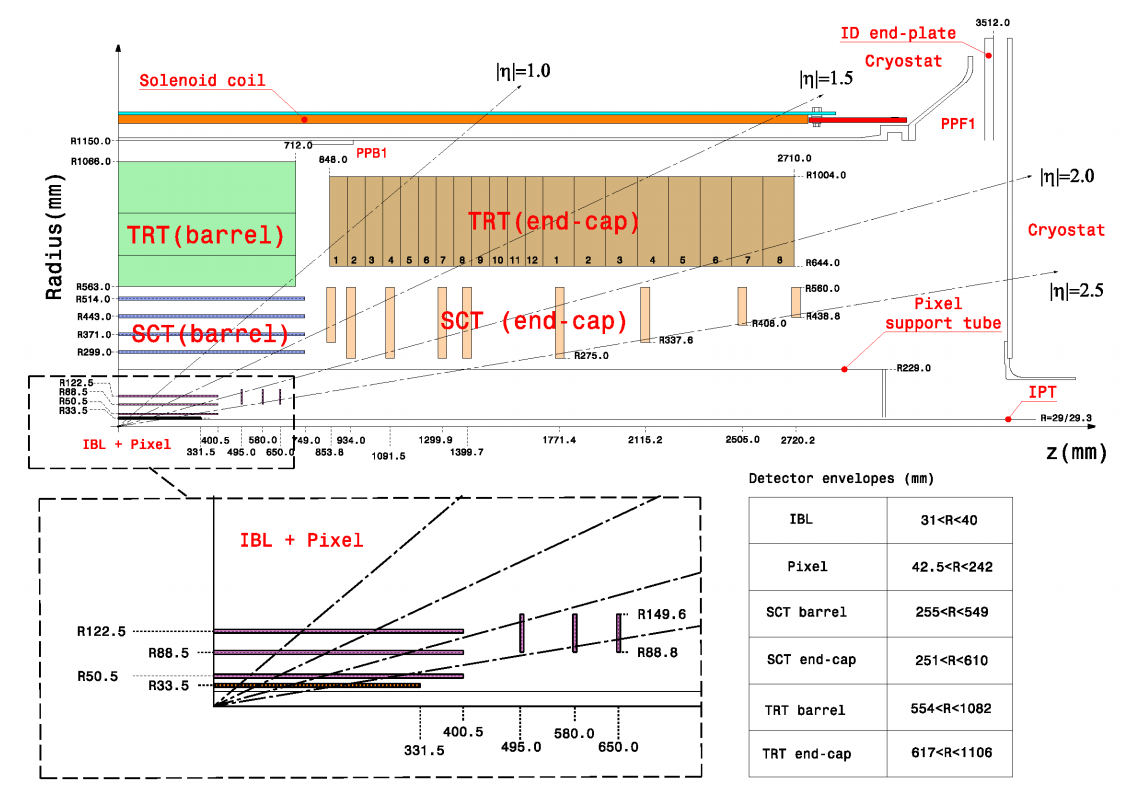
\includegraphics[width=0.9\linewidth]{figures/detector/ID}
\caption{View of a quadrant of the ATLAS inner detector in its original design (not including IBL which is inserted at $R=33.25mm$ for the Run II ATLAS experiment, Ref.\cite{SCTpaper})}
\label{fig:detector-id}
\end{center}
\end{figure}



\subsubsection{Pixel}

The pixel detector is the detector component closest to the beam line to provide best possible spatial resolution. The standard pixel sensors are bonded to readout electronics through the hybridization technique. The Run I ATLAS three pixel layers used the planar design. The size of the pixel is $50\times 400 \mu m^2$, which are limited by the size of the electronics attached to the pixels. For the Run II experiment, the collaboration decided to add another layer of pixel called insertable B-layer (IBL). Since the pixel layers are very close to the beam, radiation damage is a serious concern. The energetic particles such as neutron could knock the silicon atoms out of the lattice leading to higher bias voltage needed to deplete the bulk of the silicon as well as reducing the charge collection efficiency. At the time, a new type of pixel detector design with 3D sensor shown in Fig.\ref{fig:detector-sensor} was available. The 3D sensor collects the charge in the direction perpendicular to that of the planar sensor reducing the drifting path and hence is more radiation hard. However due to a lack of operational experience, the 3D design was only partially adopted (25\% of all the IBL sensors) and used to cover the high $|\eta|$ region (out of the $|\eta|<2.5$ active tracking regime). For the majority of the sensors, the planar design was used with the pixel size reduced to $50\times 250\mu m^2$. 

\begin{figure}[htpb!]
\begin{center}
  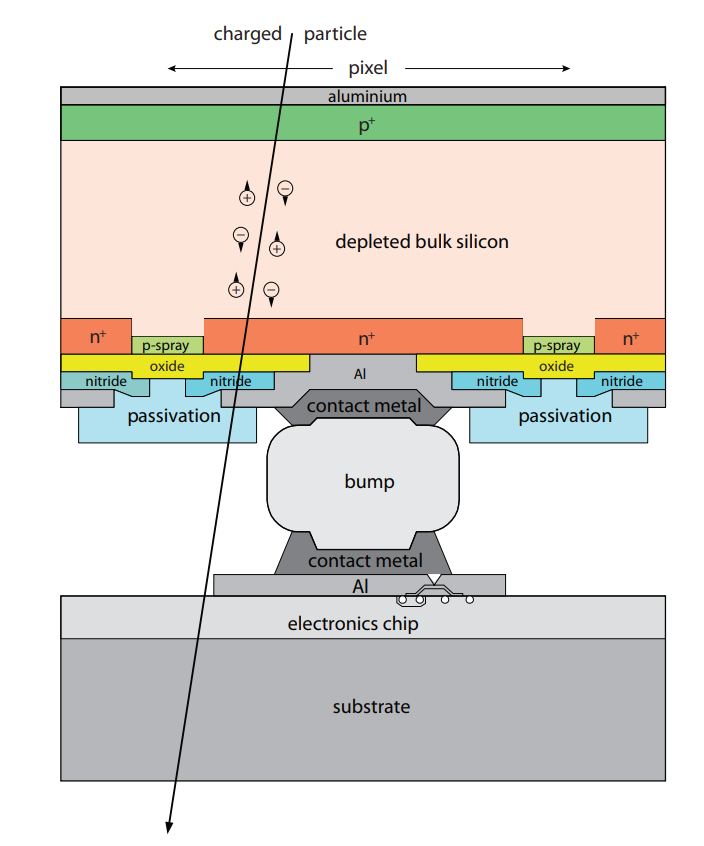
\includegraphics[width=0.35\linewidth]{figures/detector/PixelPlanar}
  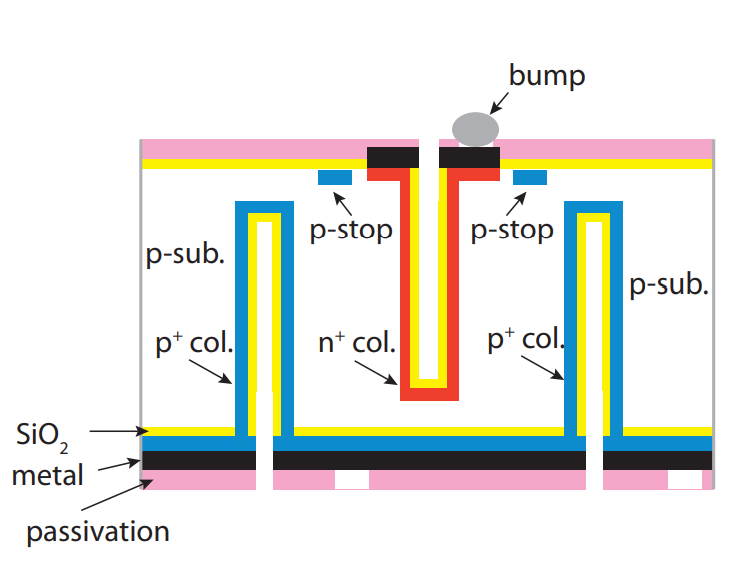
\includegraphics[width=0.40\linewidth]{figures/detector/Pixel3D}
\caption{Examples of planar (left) and 3D (right) pixel designs from \cite{PixReview}. The 3D pixel sensor design has smaller drifting path }
\label{fig:detector-sensor}
\end{center}
\end{figure}


\subsubsection{SCT}

Fabrication and manufacturing of pixel detector are difficult. Before the advent of the pixel detector, microstrips are the mainstream type of silicon trackers. The microstrips instead of reading out the two-dimensional signals directly, places two layers close to each other and reads out one-dimensional signal (hit on a strip) from both layers. The read out electronics hence can be much more simply connected to the sensors. Of course one downside of the design is the large number of ghosts when there are multiple tracks hitting the detector at the same time.

The ATLAS SCT detector adopts the microstrip design. Two sets of sensors of the same layer are rotated 40$mrad$ with respect to each other. The SCT has both the coaxial cylindrical barrel layers and disk-shaped endcap layers. The former of which has 8448 and latter has 6944 sensors\cite{SCTpaper}. Nominal design resolutions are $17\mu m$ in the $R-\phi$ plane and $580 \mu m$ in the $z$-direction \cite{PERF-2007-01}.


\subsubsection{TRT}

The outermost layer of ID is Transition Radiation Detector which serves to both find charged particle hits and identify electrons. The entire TRT consists of 298304 2mm radius straw tubes\cite{TRTpaper} as drift chambers filled with $Xe$, $CO_2$ and $O_2$ during Run I and with $Ar$, $CO_2$ and $O_2$ during Run II to collect the electrons rising from primary ionization of charged particles. In addition, polypropylene fibers with diameter of $19\mu m$ serve as the radiators. Photons emitted primarily from the transition radiations of electrons going across media of different refraction index are signals of electron identification.
